\documentclass[justified,nobib]{tufte-handout}
\usepackage{microtype}
\usepackage{amsmath}
\usepackage{graphicx}
\title{Second Order Butterworth Filter}
\author{Chris Curro}
\date{\today}
\begin{document}
\maketitle
\begin{abstract}
As per the project specification, a second order Butterworth filter was
constructed with a Sallen-Key topology. The corner frequency for this filter is
about 450~Hz meaning it could be used for surface EMG readings.
\end{abstract}
\section{Design}
\vspace{-0.2in}
\begin{figure}[h]
\centering
\label{schem}
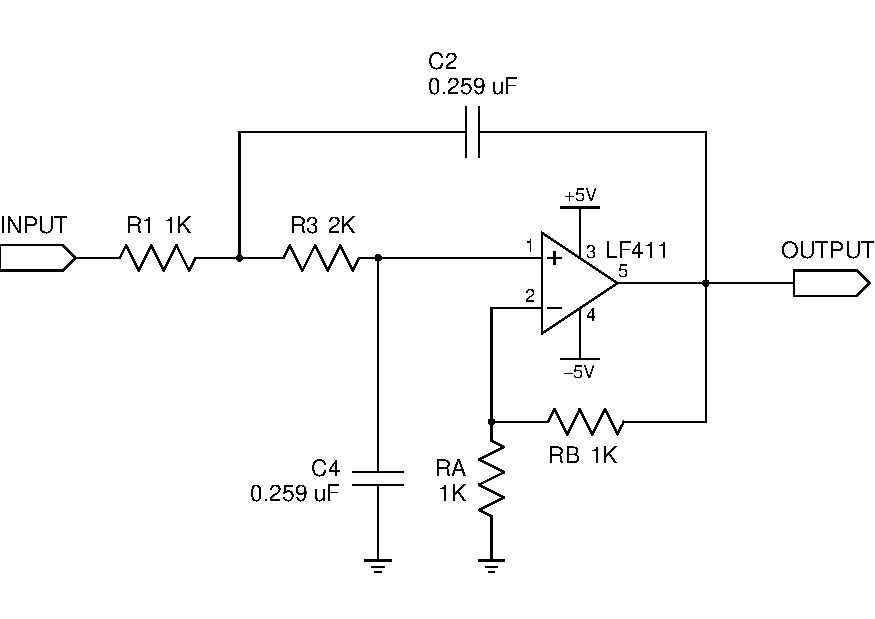
\includegraphics[width=0.9\linewidth,trim=0 .3in 0 .35in,clip=true]{schem.pdf}
\caption{Schematic for the filter.}
\end{figure}
\paragraph{} The first step in the design process was selected the appropriate
components to meet the specification. The specification for a filter useful for
surface EMG readings was a cutoff frequency less than 500~Hz. Furthermore two
constraints were set which reduced the parameter space; the two capacitors were
constrained to be of equal value and the DC voltage gain of the system was set
to be 2 (6~dB). The latter constraint imposes the condition that $R_A = R_B$ by
the equation:
\begin{equation}
K = 1 + \frac{R_B}{R_A}
\end{equation}
Combining the constraints and acknowledging the fact that this circuit is
Butterworth filter the following equation can be written for the Q-Factor:
\begin{equation}
\frac{1}{Q} = \sqrt{2} = \sqrt{\frac{R_3}{R_1}}
\end{equation}
Solving for $R_3$, a final constraint becomes evident:
\begin{equation}
R_3 = 2R_1
\end{equation}
Taking this into consideration a value of 1 k$\Omega$ was selected for $R_1$;
therefore $R_2$ is required to be 2 k$\Omega$. These values were selected
because 1 k$\Omega \pm 1\%$ resistors were available in the lab, therefore it
was easier to meet the correct ratio.
\paragraph{} The last remaining parameters were $C_2$ and $C_4$ which were
already constrained to be equal to each other (denoted as $C$). Incorporating
this constraint and the Sallen-Key topology the the parameter can be solved for
with the following equation:
\begin{equation}
2\pi f_c = \frac{1}{\sqrt{R_1R_2C^2}}
\end{equation}
With $f_c$ set by the specification, and $R_1$ and $R_2$ set above it was simple
to solve for $C$, which became 0.225 $\mu$F. The theoretical value selected
for $C$ was 0.22 $\mu$F because it was available in the lab. However because the
two capacitors present needed to be matched significant testing was required to
discover two matched capacitors. Ultimately the capacitors used had a value of
0.259 $\mu$F as measured by a RSR M9803R Multimeter. 
\paragraph{} Using the actual values of the capacitors and the selected values
for $R_1$ and $R_2$ the change the cutoff frequency was calculated to see if it
were tolerable for the design specification. The new theoretical cutoff
frequency was 434~Hz which is tolerable for surface EMG measurements, per the
specification. 
\section{Test Procedure and Results}
\paragraph{Frequency Response} The magnitude frequency response was
measured with a Hewlett Packard 35660A Dynamic Signal Analyzer from 10~Hz up to
1000~Hz. These results are summarized in Figure \ref{freqr}. An additional
measurement was made at 10 kHz to confirm that the stop band falls off at rate
of 40 dB/decade (the measurement showed a falloff of 39 dB in the decade from
1000~Hz). The first measurement was made at 10~Hz, and then at 50~Hz with
the following measurements collected up to 1000~Hz at increments of 50~Hz. The
HP 35660A was responsible for both stimulating the device under test and
measuring the response.
\begin{figure}
\centering
\label{freqr}
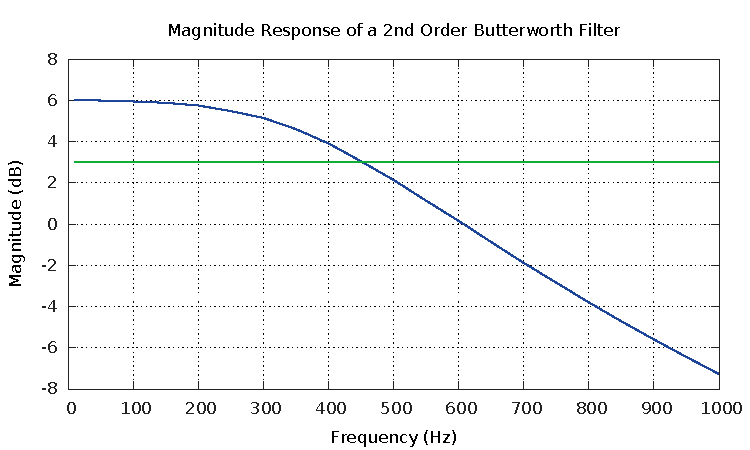
\includegraphics[width=0.81\linewidth]{magResponse.pdf}
\caption{Frequency response of the Butterworth filter}
\end{figure}
\bibliography{bib}{}
\bibliographystyle{IEEEtran}
\end{document}